% ============================================================================
%  Luxe Core AI — Presentación TFG (Beamer)
%  Autor: Jesús Fernández López — Tutor: Dr. Rafael Muñoz Salinas
%  UCO — Escuela Politécnica Superior — junio 2026
% ============================================================================
\PassOptionsToPackage{table}{xcolor}
\documentclass[11pt, spanish, aspectratio=169]{beamer}

% --- Encoding, Fuentes e Idioma ---
\usepackage[utf8]{inputenc}
\usepackage[T1]{fontenc}
\usepackage[spanish, es-tabla]{babel}
\usepackage{csquotes}
\usepackage{libertine}
\usepackage[scaled=0.85]{beramono}
\usepackage{microtype}

% --- Paquetes Esenciales ---
\usepackage{graphicx}
\usepackage{tikz}
\usepackage{booktabs}
\usepackage{array}
\usepackage{listings}
\usepackage{hyperref}
\usepackage{qrcode}
\usepackage{totcount}
\usepackage{calc}
\usepackage{multimedia}
\usepackage[skins]{tcolorbox}
\tcbuselibrary{breakable, skins}

% --- Contador total de frames ---
\regtotcounter{framenumber}

% ============================================================================
%  TCOLORBOX — Estilos de bloques personalizados (borde izquierdo accent)
% ============================================================================
\tcbset{
  luxeblock/.style={
    enhanced,
    colback=secondarylight,
    colbacktitle=primary,
    coltitle=white,
    fonttitle=\bfseries\footnotesize,
    colframe=accent,
    attach boxed title to top left={xshift=3mm, yshift=-3mm, yshifttext=-1mm},
    boxed title style={size=small, colback=primary, sharp corners, boxrule=0pt},
    drop fuzzy shadow,
    boxrule=0pt,
    leftrule=3pt,
    arc=2pt,
    left=4mm, right=3mm, top=3mm, bottom=2mm,
    before skip=2pt, after skip=15pt,
  },
  luxealert/.style={
    luxeblock,
    colbacktitle=alertred,
    colframe=alertred,
    boxed title style={size=small, colback=alertred, sharp corners, boxrule=0pt},
  },
  luxeexample/.style={
    luxeblock,
    colbacktitle=exgreen,
    colframe=exgreen,
    boxed title style={size=small, colback=exgreen, sharp corners, boxrule=0pt},
  },
}

% ============================================================================
%  PALETA DE COLORES CORPORATIVA EPSC (coherente con la memoria)
% ============================================================================
\definecolor{primary}{HTML}{280091}        % EPSCDark — violeta institucional
\definecolor{primarydark}{HTML}{1A0060}    % Más oscuro para pie
\definecolor{secondary}{HTML}{4C5CC5}      % EPSCMedium — violeta medio
\definecolor{secondarylight}{HTML}{EDEEF8} % Violeta muy claro (fondo bloques)
\definecolor{bgcolor}{HTML}{FAFAFA}        % Fondo principal
\definecolor{accent}{HTML}{3FCFD5}         % EPSCLight — verde azulado
\definecolor{exgreen}{HTML}{00B299}        % EPSCGreen — verde corporativo
\definecolor{alertred}{HTML}{C0392B}       % Rojo alerta
\definecolor{darkgray}{RGB}{80,80,80}

% ============================================================================
%  COLORES BEAMER
% ============================================================================
\setbeamercolor{structure}{fg=primary}
\setbeamercolor{background canvas}{bg=bgcolor}
\setbeamercolor{normal text}{fg=darkgray}
\setbeamercolor{frametitle}{fg=white, bg=primary}
\setbeamercolor{frametitle accent}{fg=secondary, bg=secondary}
\setbeamercolor{footline}{fg=secondary!70, bg=bgcolor}
\setbeamercolor{author in head/foot}{fg=secondarylight, bg=primarydark}
\setbeamercolor{page number in head/foot}{fg=white, bg=primarydark}
\setbeamercolor{block title}{fg=white, bg=primary}
\setbeamercolor{block body}{fg=black, bg=secondarylight}
\setbeamercolor{block title alerted}{fg=white, bg=alertred}
\setbeamercolor{block body alerted}{fg=black, bg=secondarylight}
\setbeamercolor{block title example}{fg=white, bg=exgreen}
\setbeamercolor{block body example}{fg=black, bg=secondarylight}
\setbeamercolor{itemize item}{fg=primary}
\setbeamercolor{itemize subitem}{fg=secondary}
\setbeamercolor{enumerate item}{fg=primary}
\setbeamercolor{enumerate subitem}{fg=secondary}
\setbeamercolor{section in toc}{fg=primary}
\setbeamercolor{subsection in toc}{fg=darkgray}

% ============================================================================
%  FUENTES
% ============================================================================
\setbeamerfont{frametitle}{size=\Large, series=\bfseries}
\setbeamerfont{footline}{size=\footnotesize}
\setbeamerfont{block title}{size=\normalsize, series=\bfseries}
\setbeamerfont{author in head/foot}{size=\scriptsize}
\setbeamerfont{page number in head/foot}{size=\footnotesize, series=\bfseries}

% ============================================================================
%  PLANTILLAS PERSONALIZADAS
% ============================================================================
\setbeamertemplate{navigation symbols}{}

% --- Frametitle: barra navy + triángulo accent (sin número de página) ---
\setbeamertemplate{frametitle}{%
  \nointerlineskip%
  \begin{beamercolorbox}[wd=\paperwidth, ht=2.8ex, dp=1.5ex, leftskip=0.6cm]{frametitle}%
    \hyperlink{indice}{\textcolor{accent}{\textbf{$\blacktriangleright$}}}\hspace{0.25cm}%
    \usebeamerfont{frametitle}\insertframetitle%
  \end{beamercolorbox}%
  \nointerlineskip%
  \begin{beamercolorbox}[wd=\paperwidth, ht=2.5pt, dp=0pt]{frametitle accent}%
  \end{beamercolorbox}%
}

% --- Footline: línea accent + nº página TikZ en esquina inferior derecha ---
%     Oculto en portada (frame 1) e índice (frame 2).
\setbeamertemplate{footline}{%
  \ifnum\insertframenumber<3\relax
  \else
    \begin{tikzpicture}[remember picture, overlay]
      % Línea accent inferior
      \draw[accent, line width=1.5pt]
        (current page.south west) -- (current page.south east);
      % Nº página en esquina inferior derecha (sobre la línea)
      \node[anchor=south east, xshift=-0.22cm, yshift=0.3cm,
            font=\scriptsize\color{secondary!60}]
        at (current page.south east) {\insertframenumber\ / \total{framenumber}};
    \end{tikzpicture}%
  \fi
}

% --- Bloques: tcolorbox personalizados con leftrule accent ---
\setbeamertemplate{block begin}{%
  \begin{tcolorbox}[luxeblock, title=\insertblocktitle]%
}
\setbeamertemplate{block end}{%
  \end{tcolorbox}%
}
\setbeamertemplate{block alerted begin}{%
  \begin{tcolorbox}[luxealert, title=\insertblocktitle]%
}
\setbeamertemplate{block alerted end}{%
  \end{tcolorbox}%
}
\setbeamertemplate{block example begin}{%
  \begin{tcolorbox}[luxeexample, title=\insertblocktitle]%
}
\setbeamertemplate{block example end}{%
  \end{tcolorbox}%
}

% --- Ítems ---
\setbeamertemplate{itemize items}[triangle]
\setbeamertemplate{enumerate items}[default]

% Margen extra para enumerate (evita que toque bordes)
\setlength{\leftmargini}{1.3em}
\setlength{\leftmarginii}{1em}

% Espaciado entre párrafos para separar bloques de listas
\setlength{\parskip}{0.2cm plus 2pt minus 1pt}

% --- Sin página de sección ---
\setbeamertemplate{section page}{}

% ============================================================================
%  LISTINGS — Estilo para código fuente
% ============================================================================
\lstset{
    basicstyle=\ttfamily\scriptsize,
    keywordstyle=\color{primary}\bfseries,
    commentstyle=\color{darkgray!60},
    stringstyle=\color{alertred},
    numbers=left,
    numberstyle=\tiny\color{darkgray!50},
    frame=single,
    framerule=0.6pt,
    rulecolor=\color{secondary!60},
    backgroundcolor=\color{gray!5},
    breaklines=true,
    breakatwhitespace=false,
    showstringspaces=false,
    tabsize=2,
    captionpos=b,
    aboveskip=4pt,
    belowskip=4pt,
}

% ============================================================================
%  MACROS ÚTILES
% ============================================================================
\newcommand{\memoriaimg}{../memoria/img}
\newcommand{\smallgray}[1]{\textcolor{darkgray}{\small #1}}

% ============================================================================
%  METADATOS
% ============================================================================
\title[Luxe Core AI]{Ecosistema de Domótica Local Impulsado por Agentes de IA}
\subtitle{Luxe Core AI}
\author[J. Fernández]{\textbf{Jesús Fernández López}}
\institute[UCO — EPSC]{%
    Grado en Ingeniería Informática\\
    Escuela Politécnica Superior de Córdoba\\
    Universidad de Córdoba
}
\date{Junio 2026}

% ============================================================================
%  INICIO DEL DOCUMENTO
% ============================================================================
\begin{document}

% ============================================
%  BLOQUE I — PORTADA E INTRODUCCIÓN  (1–3)
% ============================================
% ============================================================================
%  BLOQUE I — DIAPOSITIVA 1: PORTADA
% ============================================================================
{
\setbeamertemplate{footline}{}
\setbeamertemplate{frametitle}{}
\setbeamertemplate{headline}{}

\begin{frame}[plain]

  \begin{tikzpicture}[remember picture, overlay]

    % --- Esquina superior derecha (decoración institucional) ---
    \node[anchor=north east, inner sep=0pt] at (current page.north east) {%
      \IfFileExists{\memoriaimg/topRightCorner.pdf}{%
        
\includegraphics[width=2.5cm]{\memoriaimg/topRightCorner.pdf}%
      }{}%
    };

    % --- Esquina inferior izquierda (decoración institucional) ---
    \node[anchor=south west, inner sep=0pt] at (current page.south west) {%
      \IfFileExists{\memoriaimg/bottomLeftCorner.pdf}{%
        
\includegraphics[width=2.5cm]{\memoriaimg/bottomLeftCorner.pdf}%
      }{}%
    };

    % --- Escudo Informática + Logo UCO (esquina inferior derecha) ---
    \node[anchor=south east, xshift=-0.8cm, yshift=0.8cm] at (current page.south east) {%
      \IfFileExists{\memoriaimg/escudo_informatica.jpg}{%
        
\includegraphics[height=1.0cm]{\memoriaimg/escudo_informatica.jpg}%
      }{}%
      \hspace{0.2cm}%
      \IfFileExists{\memoriaimg/logoUCO.pdf}{%
        
\includegraphics[height=1.0cm]{\memoriaimg/logoUCO.pdf}%
      }{}%
    };

    % --- Línea decorativa en accent (borde superior sutil) ---
    \draw[accent, line width=3pt]
      (current page.north west) -- (current page.north east);

  \end{tikzpicture}

  % --- Contenido textual ---
  \vspace*{0.5cm}

  {\parskip=0pt
  \begin{center}

    \IfFileExists{\memoriaimg/LogotipoEPSC.pdf}{%
      
\includegraphics[width=5cm]{\memoriaimg/LogotipoEPSC.pdf}%
    }{%
      \textcolor{primary}{\Huge\bfseries EPSC — UCO}%
    }

    \vspace{0.3cm}

    {\normalsize\bfseries\color{primary}TRABAJO DE FIN DE GRADO}

    \vspace{0.15cm}
    \rule{0.45\textwidth}{0.5pt}

    \vspace{0.15cm}
    {\LARGE\bfseries\color{primary}
     Ecosistema de Domótica Local\\[0.06cm]
     Impulsado por Agentes de IA}

    \vspace{0.15cm}
    \rule{0.45\textwidth}{0.5pt}

    \vspace{0.15cm}
    {\large\color{secondary}\bfseries Luxe Core AI}

    \vfill

    \begin{minipage}{0.45\textwidth}
      \begin{flushleft}
        {\footnotesize\bfseries Autor:} {\normalsize Jesús Fernández López}\\[0.15cm]
        {\footnotesize\bfseries Titulación:} {\footnotesize Grado en Ing. Informática}
      \end{flushleft}
    \end{minipage}
    \hfill
    \begin{minipage}{0.45\textwidth}
      \begin{flushright}
        {\footnotesize\bfseries Tutor:} {\normalsize Dr. Rafael Muñoz Salinas}
      \end{flushright}
    \end{minipage}

    \vfill

    \makebox[3cm]{\hrulefill}

    \vspace{0.15cm}
    {\footnotesize\color{darkgray}Universidad de Córdoba — EPSC}\\[0.06cm]
    {\footnotesize\color{darkgray}Córdoba, junio de 2026}

    \vspace*{0.22cm}
  \end{center}}

\end{frame}
}

% ============================================================================
%  BLOQUE I — DIAPOSITIVAS 2–3: ÍNDICE + INTRODUCCIÓN
% ============================================================================

% ----------------------------------------------------------------------------
%  DIAPOSITIVA 2 — ÍNDICE
% ----------------------------------------------------------------------------
{
\setbeamertemplate{footline}{}
\begin{frame}{Índice}
  \hypertarget{indice}{}%
  \tableofcontents
\end{frame}
}

\section{Introducción}

% ----------------------------------------------------------------------------
%  DIAPOSITIVA 3 — RESUMEN EJECUTIVO + MOTIVACIÓN
% ----------------------------------------------------------------------------
\begin{frame}{Resumen Ejecutivo y Motivación}
  \begin{columns}[T]
    \column{0.48\textwidth}
    \IfFileExists{figures/03_arquitectura.pdf}{%
      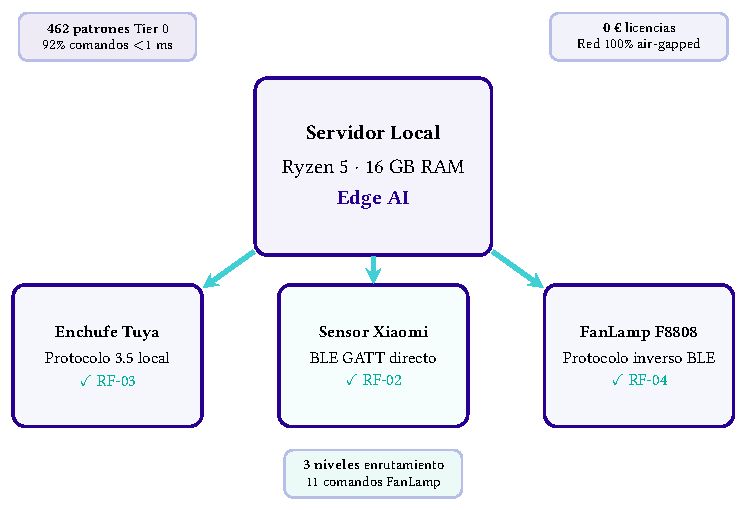
\includegraphics[width=\textwidth, height=3.8cm, keepaspectratio]{figures/03_arquitectura.pdf}%
    }{
      \textcolor{darkgray}{[Figura: panorama del sistema]}
    }

    \vspace{0.15cm}
    \begin{block}{¿Qué es Luxe Core AI?}
      \footnotesize
      Sistema 100\% local de control de confort térmico orquestado por IA en el \textit{edge}.
      \textbf{462 patrones} Tier~0 (92\%, $<$1 ms) · \textbf{0 €} licencias · Red air-gapped.
    \end{block}

    \column{0.52\textwidth}
    \IfFileExists{figures/04_motivacion.pdf}{%
      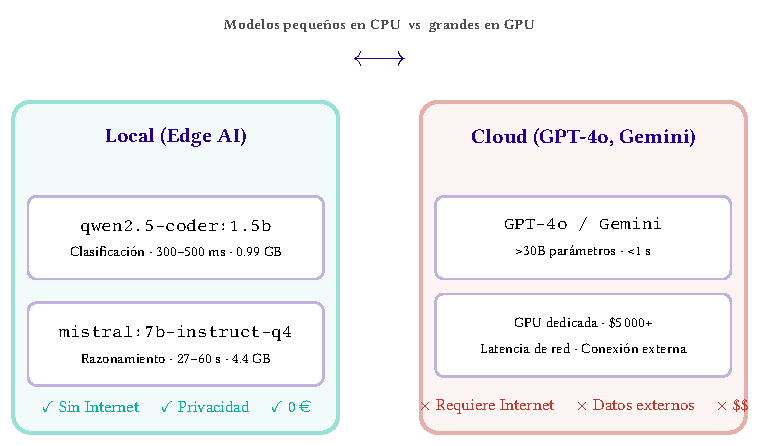
\includegraphics[width=\textwidth, height=3.8cm, keepaspectratio]{figures/04_motivacion.pdf}%
    }{
      \textcolor{darkgray}{[Figura: comparativa Local vs Cloud]}
    }

    \vspace{0.15cm}
    \begin{exampleblock}{Principio rector}
      \footnotesize
      La tecnología del hogar no debería exigir ceder la privacidad a cambio de comodidad.
    \end{exampleblock}
  \end{columns}
\end{frame}


% ============================================
%  BLOQUE II — PROBLEMA Y OBJETIVOS  (4–6)
% ============================================
% ============================================================================
%  BLOQUE II — DIAPOSITIVAS 4–6: PROBLEMA Y OBJETIVOS
% ============================================================================
\section{Problema y Objetivos}

% ----------------------------------------------------------------------------
%  DIAPOSITIVA 4 — PROBLEMA + OBJETIVO GENERAL (fusionada)
% ----------------------------------------------------------------------------
\begin{frame}{Problema y Objetivo General}
  \hypertarget{s:problema}{}
  \begin{columns}[T]
    \column{0.5\textwidth}
    \begin{alertblock}{El problema}
      \footnotesize
      La domótica actual depende de servicios cloud: sin Internet,
      el hogar inteligente se vuelve inerte. Los datos de comportamiento
      viajan a servidores de terceros.
    \end{alertblock}

    \begin{exampleblock}{La respuesta}
      \footnotesize
      Sistema 100\% local de control de confort térmico orquestado
      por IA en el \textit{edge}. Interoperabilidad real sin modificar hardware.
    \end{exampleblock}

    \column{0.5\textwidth}
    \begin{block}{Objetivo general}
      \centering
      Diseñar, implementar y validar un sistema de monitorización
      y control de confort térmico que opere de forma autónoma
      en una red local privada, eliminando cualquier dependencia
      de servicios en la nube.
    \end{block}
  \end{columns}

  \vspace{0.4cm}
  \begin{columns}[T]
    \column{0.33\textwidth}
    \centering
    \textcolor{primary}{\textbf{Coste cero}}\\[0.1cm]
    {\footnotesize 0 € en licencias, APIs externas o suscripciones}
    \column{0.33\textwidth}
    \centering
    \textcolor{primary}{\textbf{Reproducibilidad}}\\[0.1cm]
    {\footnotesize Mismo hardware $\rightarrow$ replicar con la documentación}
    \column{0.33\textwidth}
    \centering
    \textcolor{primary}{\textbf{Hardware real}}\\[0.1cm]
    {\footnotesize Pruebas sobre dispositivos físicos, no simulación}
  \end{columns}
\end{frame}

% ----------------------------------------------------------------------------
%  DIAPOSITIVA 6 — OBJETIVOS ESPECÍFICOS E INDICADORES
% ----------------------------------------------------------------------------
\begin{frame}{Objetivos Específicos e Indicadores}
  \hypertarget{s:objetivos}{}
  \centering
  \IfFileExists{figures/08_objetivos.pdf}{%
    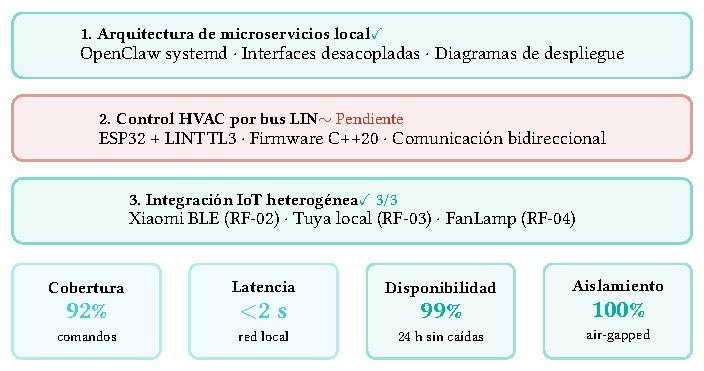
\includegraphics[width=0.92\textwidth, height=5.5cm, keepaspectratio]{figures/08_objetivos.pdf}%
  }{
    \textcolor{darkgray}{[Figura: dashboard de objetivos]}
  }
\end{frame}


% ============================================
%  BLOQUE III — RESTRICCIONES Y METODOLOGÍA  (7–10)
% ============================================
% ============================================================================
%  BLOQUE III — DIAPOSITIVAS 8–11: RESTRICCIONES Y METODOLOGÍA
% ============================================================================
\section{Restricciones y Metodología}

% ----------------------------------------------------------------------------
%  DIAPOSITIVA 8 — FACTORES DE DISEÑO
% ----------------------------------------------------------------------------
\begin{frame}{Restricciones y Factores de Diseño}
  \begin{columns}[T]
    \column{0.5\textwidth}
    \begin{alertblock}{Restricción temporal y económica}
      \footnotesize
      \begin{itemize}
        \item Un curso académico $\rightarrow$ MVP con funcionalidades troncales
        \item Autor: estudiante sin ingresos — presupuesto \textbf{56,50 €}
        \item Ingeniería inversa como alternativa a la inversión
      \end{itemize}
    \end{alertblock}

    \column{0.5\textwidth}
    \begin{exampleblock}{Impacto positivo}
      \footnotesize
      \begin{itemize}
        \item Obliga a desarrollar competencias transferibles
        \item GATT Xiaomi sin autenticación: una herramienta cara lo habría ocultado
        \item Domótica inteligente $\neq$ grandes inversiones
      \end{itemize}
    \end{exampleblock}

    \begin{block}{Evolución de infraestructura}
      \footnotesize
      \textbf{Fase 1:} servidores UCO con GPU (prototipado)\\
      \textbf{Fase 2:} torre Ryzen 5, 16 GB RAM, 100\% local
    \end{block}
  \end{columns}
\end{frame}

% ----------------------------------------------------------------------------
%  DIAPOSITIVA 9 — PERÍMETRO AIR-GAPPED
% ----------------------------------------------------------------------------
\begin{frame}{Arquitectura de Red Air-Gapped}
  \begin{columns}[T]
    \column{0.5\textwidth}
    \footnotesize
    \textbf{Problema:} los dispositivos comerciales intentan abrir canales hacia sus nubes.

    \textbf{Solución: Router sin salida WAN}
    \begin{itemize}
      \item TP-Link TL-MR6400 sin tarjeta SIM
      \item Actúa como \textit{switch} Ethernet + AP WLAN
      \item Segmento \texttt{192.168.1.0/24} completamente aislado
      \item IPs estáticas — aislamiento físico verificable
    \end{itemize}

    \column{0.5\textwidth}
    \begin{exampleblock}{Propiedades del segmento aislado}
      \footnotesize
      \begin{itemize}
        \item \textbf{Topología plana:} todos los dispositivos en \texttt{192.168.1.0/24}
        \item \textbf{IPs estáticas} sin DHCP — sin dependencias externas
        \item \textbf{Un solo router:} TL-MR6400 sin tarjeta SIM
        \item \textbf{Sin puerta de enlace WAN:} el tráfico no puede salir
        \item \textbf{Verificable:} retirar la SIM demuestra el diseño
      \end{itemize}
    \end{exampleblock}
  \end{columns}
\end{frame}

% ----------------------------------------------------------------------------
%  DIAPOSITIVA 10 — STACK POLÍGLOTA
% ----------------------------------------------------------------------------
\begin{frame}{Stack Políglota y Justificación}
  \begin{block}{Principio}
    \small
    La naturaleza dual de la domótica con IA (tiempo real + flexibilidad cognitiva)
    hace inviable un sistema monolítico en un solo lenguaje.
  \end{block}

  \begin{columns}[T]
    \column{0.33\textwidth}
    \begin{exampleblock}{Python 3.12}
      \footnotesize
      \textbf{Drivers de dispositivos}\\[0.05cm]
      \texttt{tinytuya}, \texttt{bleak}\\[0.1cm]
      \textbf{Enrutador de modelos}\\[0.05cm]
      HTTP server, comfort advisors\\[0.1cm]
      $\rightarrow$ Ecosistema maduro, prototipado rápido
    \end{exampleblock}

    \column{0.33\textwidth}
    \begin{exampleblock}{Node.js 24}
      \footnotesize
      \textbf{Orquestador OpenClaw} \smallgray{(externo)}\\[0.05cm]
      Canales Telegram y dashboard web\\[0.1cm]
      Interfaz de agentes IA\\[0.05cm]
      \texttt{exec} $\rightarrow$ drivers Python\\[0.1cm]
      $\rightarrow$ Gestión nativa de canales
    \end{exampleblock}

    \column{0.33\textwidth}
    \begin{block}{C++20}
      \footnotesize
      \textbf{Firmware ESP32}\\[0.05cm]
      Control determinista de memoria\\[0.1cm]
      Bus LIN \smallgray{(pendiente)}\\[0.1cm]
      $\rightarrow$ \textit{Hard real-time} cuando se necesita
    \end{block}
  \end{columns}

  \centering
  \footnotesize
  Cada lenguaje en su capa óptima, sin acoplar tiempos de ejecución ni forzar compromisos.
\end{frame}

% ----------------------------------------------------------------------------
%  DIAPOSITIVA 11 — METODOLOGÍA DOCS-AS-CODE
% ----------------------------------------------------------------------------
\begin{frame}[fragile]{Metodología: Docs-as-Code y Git}
  \begin{columns}[T]
    \column{0.5\textwidth}
    \small
    \textbf{Control de versiones}
    \begin{itemize}
      \item Repositorio privado GitHub
      \item Cada contribución auditada
      \item Trazabilidad: decisión de diseño $\leftrightarrow$ código
      \item Base para futura iniciativa empresarial
    \end{itemize}

    \bigskip
    \textbf{Docs as Code}
    \begin{itemize}
      \item Memoria \LaTeX{} + código en mismo repo
      \item Consistencia tipográfica profesional
      \item 9 ADR (\textit{Architecture Decision Records})
      \item Diagramas TikZ versionados
    \end{itemize}

    \column{0.5\textwidth}
    \footnotesize
    \textbf{Uso de IA en el desarrollo}
    \begin{itemize}
      \item \textbf{OpenCode:} asistente de codificación (software libre)
      \item \textbf{DeepSeek V4:} modelo de inferencia vía API
      \item \alert{Toda línea revisada y validada por el autor}
    \end{itemize}

    \begin{exampleblock}{Herramientas de gestión}
      SSH con llaves RSA, Cockpit (puerto 9090), \texttt{systemd}.
    \end{exampleblock}
  \end{columns}
\end{frame}


% ============================================
%  BLOQUE IV — ESPECIFICACIÓN DEL SISTEMA  (11–16)
% ============================================
% ============================================================================
%  BLOQUE IV — DIAPOSITIVAS XX–XX: ESPECIFICACIÓN DEL SISTEMA
% ============================================================================
\section{Especificación del Sistema}

% ----------------------------------------------------------------------------
%  DIAPOSITIVA XX — ARQUITECTURA DE 3 CAPAS
% ----------------------------------------------------------------------------
\begin{frame}{Arquitectura de 3 Capas}
  \hypertarget{s:arquitectura}{}
  \begin{columns}[T]
    \column{0.48\textwidth}
    \footnotesize
    \textbf{Servidor de orquestación}
    \begin{itemize}
      \item Torre Ryzen 5, 16 GB RAM, Ubuntu Server headless
      \item OpenClaw Gateway (Node.js 24, puerto 18789)
      \item Ollama: qwen2.5 1.5B + mistral 7B + bge-m3
      \item Drivers Python (Tuya, BLE, FanLamp)
    \end{itemize}

    \textbf{Nodo firmware}
    \begin{itemize}
      \item ESP32 — puente BLE FanLamp
      \item \smallgray{Futuro: LIN HVAC con el mismo hardware}
    \end{itemize}

    \column{0.52\textwidth}
    \IfFileExists{\memoriaimg/fig_8_1.pdf}{%
      
\includegraphics[width=\textwidth, height=5.8cm, keepaspectratio]{\memoriaimg/fig_8_1.pdf}%
    }{%
      \fbox{\parbox{0.9\textwidth}{\centering\footnotesize [Diagrama de arquitectura]}}%
    }
  \end{columns}

  \centering
  \footnotesize
  Comunicación exclusiva sobre \texttt{192.168.1.0/24}. Ningún dato abandona el perímetro local.
\end{frame}

% ----------------------------------------------------------------------------
%  DIAPOSITIVA XX — MODEL ROUTER V2
% ----------------------------------------------------------------------------
\begin{frame}{Model Router v2: Enrutamiento en 3 Niveles}
  \hypertarget{s:router}{}
  \sloppy
  \begin{columns}[T]
    \column{0.03\textwidth}
    \column{0.63\textwidth}
    \centering
    \IfFileExists{figures/13_router.pdf}{%
      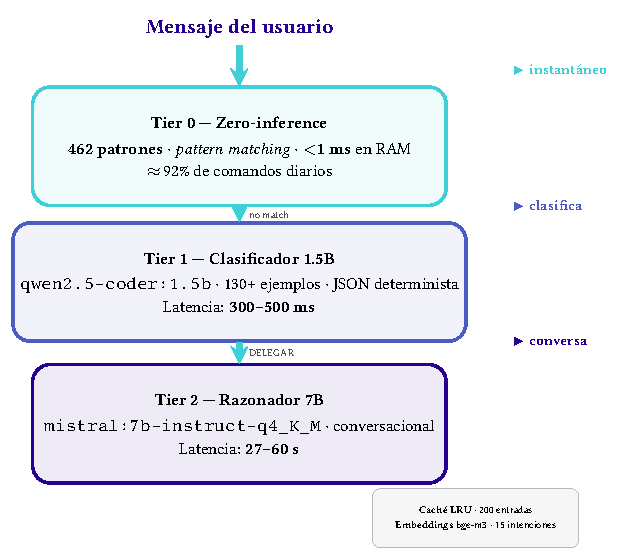
\includegraphics[width=\textwidth, height=5.8cm, keepaspectratio]{figures/13_router.pdf}%
    }{
      \textcolor{darkgray}{[Figura: flujo del Model Router v2]}
    }

    \column{0.31\textwidth}
    \centering
    \footnotesize
    \textbf{Ejemplos}\\[0.15cm]
    \renewcommand{\arraystretch}{1.1}
    \begin{tabular}{p{0.9cm}p{0.7cm}p{0.7cm}}
      \toprule
      \textbf{Com.} & \textbf{Niv.} & \textbf{Lat.} \\
      \midrule
      «vel.3» & T0 & 1,5 s \\
      «casa» & T0 & $<$1 ms \\
      «enciende» & T1 & 300 ms \\
      «buenos días» & T2 & 27--60 s \\
      \bottomrule
    \end{tabular}

    \vspace{0.3cm}
    \begin{alertblock}{Circuit Breaker}
      \footnotesize
      Si el 1.5B falla, deriva al Tier~2.
    \end{alertblock}
    \column{0.03\textwidth}
  \end{columns}
\end{frame}

% ----------------------------------------------------------------------------
%  DIAPOSITIVA XX — COMPARATIVA DE MODELOS
% ----------------------------------------------------------------------------
\begin{frame}{Selección de Modelos: Pruebas y Decisión}
  \hypertarget{s:modelos}{}
  \begin{columns}[T]
    \column{0.5\textwidth}
    \begin{block}{Proceso de evaluación}
      \footnotesize
      \textbf{Tres fases de pruebas} sobre Ryzen 5 (16 GB RAM, sin GPU)
      \begin{itemize}
        \item Corpus de 500 comandos reales
        \item Modelos probados: Qwen2.5 1.5B, Mistral 7B, Qwen3.5 4B
        \item Criterios: latencia, fiabilidad, consumo de recursos
      \end{itemize}
    \end{block}

    \begin{alertblock}{Qwen3.5: no viable en CPU}
      \footnotesize
      Versión reciente con modo \textit{thinking} forzado (no opcional).
      Resultado: 3--12 min por consulta en CPU. Diseñado para GPU.
    \end{alertblock}

    \column{0.5\textwidth}
    \begin{exampleblock}{Arquitectura seleccionada}
      \footnotesize
      \textbf{Tier 1 — Qwen2.5 1.5B} (determinista)
      \begin{itemize}
        \item 0,3--0,5 s por consulta
        \item Clasificación de comandos
      \end{itemize}
      \textbf{Tier 2 — Mistral 7B Q4} (conversacional)
      \begin{itemize}
        \item 27--60 s por consulta
        \item Razonamiento complejo
      \end{itemize}
    \end{exampleblock}

    \begin{block}{Ventaja clave}
      \footnotesize
      \textbf{Model-agnostic:} la arquitectura permite cambiar
      modelos sin modificaciones. Si un modelo futuro funciona
      mejor en CPU, se integra directamente.
    \end{block}
  \end{columns}
\end{frame}

% ----------------------------------------------------------------------------
%  DIAPOSITIVA XX — COMFORT ADVISORS
% ----------------------------------------------------------------------------
\begin{frame}{Asesores de Confort Térmico}
  \hypertarget{s:confort}{}
  \begin{columns}[T]
    \column{0.5\textwidth}
    \begin{block}{Evaluación del confort}
      \footnotesize
      El sistema evalúa continuamente:
      \begin{itemize}
        \item Condiciones interiores (temperatura, humedad)
        \item Condiciones exteriores (clima, radiación solar)
        \item Presencia de usuarios
      \end{itemize}
    \end{block}

    \column{0.5\textwidth}
    \begin{exampleblock}{Toma de decisiones}
      \footnotesize
      Basado en umbrales definidos:
      \begin{itemize}
        \item Sugiere acciones al usuario
        \item Ejecuta automáticamente si el usuario acepta
        \item Respeta siempre la decisión del usuario
      \end{itemize}
    \end{exampleblock}
  \end{columns}

  \vspace{0.5cm}
  \begin{alertblock}{Principio clave}
    \centering\footnotesize
    El sistema sugiere, el usuario decide.
  \end{alertblock}
\end{frame}

% ----------------------------------------------------------------------------
%  DIAPOSITIVA XX — AUTO-RECUPERACIÓN
% ----------------------------------------------------------------------------
\begin{frame}{Auto-Recuperación y Tolerancia a Fallos}
  \hypertarget{s:recuperacion}{}
  \centering
  \begin{columns}[T]
    \column{0.48\textwidth}
    \centering
    \IfFileExists{figures/17_recuperacion.pdf}{%
      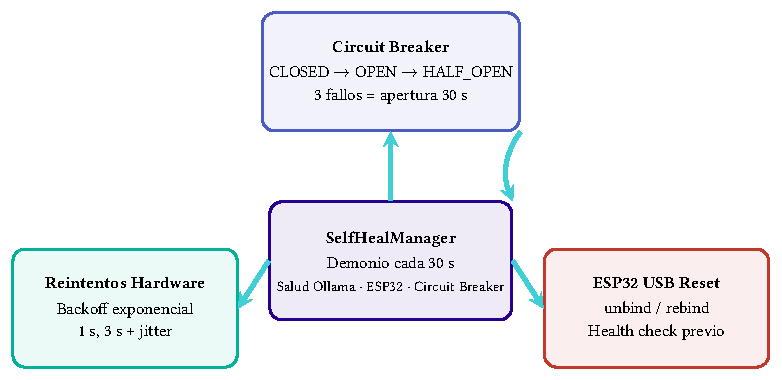
\includegraphics[width=\textwidth, height=4.5cm, keepaspectratio]{figures/17_recuperacion.pdf}%
    }{
      \textcolor{darkgray}{[Figura: ciclo de auto-recuperación]}
    }

    \column{0.48\textwidth}
    \begin{exampleblock}{Flujo de recuperación}
      \scriptsize
      \textbf{SelfHealManager} verifica cada 30\,s la salud de
      Ollama, Circuit Breaker y ESP32. Ante un fallo:
      \begin{enumerate}
        \item \textbf{Circuit Breaker} aísla el servicio
              (\texttt{CLOSED} $\to$ \texttt{OPEN})
        \item \textbf{Reintentos} con backoff + jitter (1\,s, 3\,s)
        \item Si persiste: \textbf{reset USB} del ESP32
      \end{enumerate}
      Sin intervención humana.
    \end{exampleblock}
  \end{columns}
\end{frame}


% ============================================
%  BLOQUE V — INTEGRACIÓN DE HARDWARE  (17–20)
% ============================================
% ============================================================================
%  BLOQUE V — DIAPOSITIVAS 18–21: INTEGRACIÓN DE HARDWARE
% ============================================================================
\section{Integración de Hardware}

% ----------------------------------------------------------------------------
%  DIAPOSITIVA 18 — TUYA + HOTSPOT SPOOFING
% ----------------------------------------------------------------------------
\begin{frame}{5 — Integración Tuya: Control Local y Hotspot Spoofing}
  \hypertarget{s:tuya}{}

  \IfFileExists{figures/19_tuya.pdf}{%
    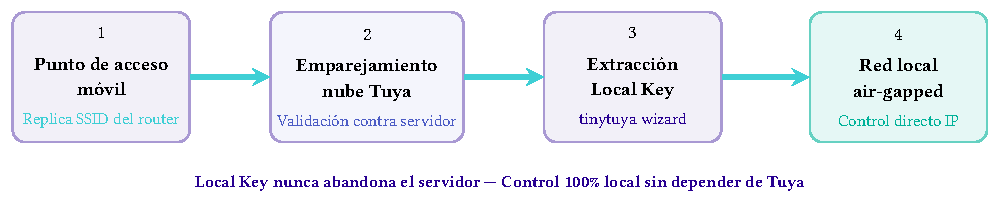
\includegraphics[width=\textwidth, height=4.2cm, keepaspectratio]{figures/19_tuya.pdf}%
  }{
    \textcolor{darkgray}{[Figura: 4 pasos Hotspot Spoofing]}
  }

  \vspace{0.3cm}
  \begin{columns}[T]
    \column{0.35\textwidth}
    \IfFileExists{\memoriaimg/hw_tuya_plug.png}{%
      
\includegraphics[height=3cm, keepaspectratio]{\memoriaimg/hw_tuya_plug.png}%
    }{
      \fbox{\parbox{0.8\textwidth}{\centering\footnotesize [Enchufe Tuya]}}
    }

    \column{0.65\textwidth}
    \footnotesize
    \textbf{Protocolo \texttt{tinytuya} 3.5}\\
    Local Key en servidor · Respuesta $<$2 s\\
    Control ON/OFF validado en red air-gapped
  \end{columns}
\end{frame}

% ----------------------------------------------------------------------------
%  DIAPOSITIVA 19 — BLE XIAOMI GATT
% ----------------------------------------------------------------------------
\begin{frame}{5 — Sensores BLE Xiaomi: Lectura GATT Directa}
  \hypertarget{s:xiaomi}{}
  \begin{columns}[T]
    \column{0.58\textwidth}
    \centering
    \IfFileExists{\memoriaimg/fig_8_5.pdf}{%
      
\includegraphics[width=\textwidth, height=5.5cm, keepaspectratio]{\memoriaimg/fig_8_5.pdf}%
    }{%
      \fbox{\parbox{0.9\textwidth}{\centering\footnotesize [Decodificación BLE]}}
    }

    \column{0.42\textwidth}
    \centering
    \IfFileExists{\memoriaimg/hw_xiaomi_sensor.png}{%
      
\includegraphics[height=3.5cm, keepaspectratio]{\memoriaimg/hw_xiaomi_sensor.png}%
    }{
      \fbox{\parbox{0.6\textwidth}{\centering\tiny [Sensor]}}
    }\\[0.1cm]
    {\footnotesize Xiaomi LYWSD03MMC}

    \vspace{0.1cm}
    \begin{exampleblock}{Lectura GATT directa}
      \footnotesize
      Decodificación de temperatura, humedad y batería\\
      directamente del sensor, sin \textit{bind key} · Sin nube Xiaomi
    \end{exampleblock}
  \end{columns}
\end{frame}

% ----------------------------------------------------------------------------
%  DIAPOSITIVA 20 — FANLAMP: INGENIERÍA INVERSA
% ----------------------------------------------------------------------------
\begin{frame}{5 — FanLamp F8808: Ingeniería Inversa del Protocolo}
  \hypertarget{s:fanlamp}{}

  \centering
  \IfFileExists{figures/21_fanlamp.pdf}{%
    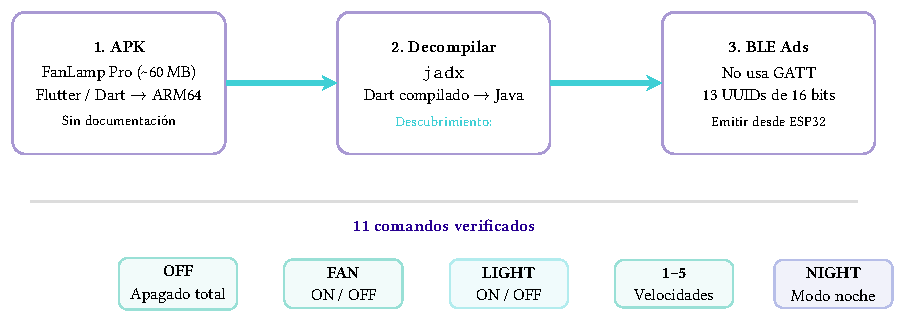
\includegraphics[width=\textwidth, height=3.8cm, keepaspectratio]{figures/21_fanlamp.pdf}%
  }{
    \textcolor{darkgray}{[Figura: ingeniería inversa FanLamp]}
  }

  \vspace{0.2cm}
  \begin{columns}[T]
    \column{0.35\textwidth}
    \IfFileExists{\memoriaimg/hw_fanlamp.png}{%
      
\includegraphics[height=2.8cm, keepaspectratio]{\memoriaimg/hw_fanlamp.png}%
    }{
      \fbox{\parbox{0.8\textwidth}{\centering\footnotesize [FanLamp F8808]}}
    }\\[0.05cm]
    {\footnotesize Mikomika F8808 — 35 € AliExpress}

    \column{0.65\textwidth}
    \footnotesize
    \begin{exampleblock}{Descubrimiento clave}
      APK FanLamp Pro decompilado (\texttt{jadx})\\
      \alert{No usa GATT, sino anuncios BLE}\\
      11 comandos mapeados — emitidos desde ESP32 vía USB
    \end{exampleblock}
  \end{columns}
  \vspace*{-0.2pt}
\end{frame}


% ============================================
%  BLOQUE VI — VALIDACIÓN Y PRUEBAS  (21–22)
% ============================================
% ============================================================================
%  BLOQUE VI — DIAPOSITIVAS 23–24: VALIDACIÓN Y PRUEBAS
% ============================================================================
\section{Validación y Pruebas}

% ----------------------------------------------------------------------------
%  DIAPOSITIVA 23 — SUITE DE PRUEBAS
% ----------------------------------------------------------------------------
\begin{frame}[fragile]{Suite de Pruebas: 500 Comandos}
  \begin{columns}[T]
    \column{0.55\textwidth}
    \footnotesize
    \textbf{Pruebas realizadas (hardware real):}
    \vspace{0.15cm}
    \begin{enumerate}
      \item \textbf{Tuya:} conectividad IP, ON/OFF, alternancia $\rightarrow$ \checkmark
      \item \textbf{BLE Xiaomi:} descubrimiento, GATT, decodificación $\rightarrow$ \checkmark
      \item \textbf{FanLamp:} 11 comandos verificados físicamente $\rightarrow$ \checkmark
      \item \textbf{Sensor Daemon:} lectura cada 60 s, JSON atómico $\rightarrow$ \checkmark
      \item \textbf{Model Router:} 3 niveles validados $\rightarrow$ \checkmark
      \item \textbf{Circuit Breaker:} fallo simulado + recuperación $\rightarrow$ \checkmark
    \end{enumerate}

    \column{0.45\textwidth}
    \footnotesize
    \textbf{Cobertura Tier~0 (500 comandos):}
    \vspace{0.15cm}
    \begin{itemize}
      \item Iluminación (35 variantes): 100\%
      \item Ventilador (50 variantes): 100\%
      \item Escenas (40 variantes): 100\%
      \item Consultas estado (15 variantes): 100\%
      \item Conversacionales $\rightarrow$ Tier~2: esperado
    \end{itemize}

    \begin{exampleblock}{Suite automatizada}
      \footnotesize
      \texttt{tests/test\_integration.py}\\
      5 subsistemas verificados de forma coordinada.
      No destructiva: solo comandos de lectura.
    \end{exampleblock}
  \end{columns}
\end{frame}

% ----------------------------------------------------------------------------
%  DIAPOSITIVA 24 — RESULTADOS LATENCIA
% ----------------------------------------------------------------------------
\begin{frame}{Resultados: Latencia y Cobertura}
  \sloppy
  \begin{columns}[T]
    \column{0.48\textwidth}
    \centering
    \footnotesize\setlength{\tabcolsep}{3pt}
    \resizebox{\columnwidth}{!}{%
    \begin{tabular}{lccc}
      \toprule
      \textbf{Escenario} & \textbf{Antes} & \textbf{Ahora} & \textbf{Modelo} \\
      \midrule
      «velocidad 3» & $\sim$2 s & $\sim$1,5 s & Tier~0 \\
      «cómo está la casa» & $\sim$2 s & 0--1 ms & Tier~0 \\
      «me enciendes la luz» & $\sim$3 s & $\sim$300 ms & 1.5B \\
      «buenos días» & $\sim$12 s & 27--60 s & Mistral 7B \\
      «temperatura» & 18 s & 0--1 ms & Daemon \\
      \bottomrule
    \end{tabular}%
    }

    \vspace{0.3cm}
    \IfFileExists{\memoriaimg/fig_9_2.pdf}{%
      
\includegraphics[height=2.5cm, keepaspectratio]{\memoriaimg/fig_9_2.pdf}%
    }{%
      \fbox{\parbox{0.9\textwidth}{\centering\footnotesize [Cobertura Tier 0]}}%
    }

    \column{0.52\textwidth}
    \IfFileExists{\memoriaimg/fig_9_1.pdf}{%
      
\includegraphics[height=3.2cm, keepaspectratio]{\memoriaimg/fig_9_1.pdf}%
    }{%
      \fbox{\parbox{0.9\textwidth}{\centering\footnotesize [Gráfico latencia]}}%
    }

    \begin{block}{Disponibilidad}
      \footnotesize\centering
      \texttt{model-router} \quad \texttt{sensor-daemon} \quad \texttt{openclaw-gateway}\\[0.1cm]
      \textbf{Operativos 24 h sin caídas.}
    \end{block}
  \end{columns}
\end{frame}


% ============================================
%  BLOQUE VII — DEMOSTRACIÓN Y VÍDEO  (23–24)
% ============================================
% ============================================================================
%  BLOQUE VII — DIAPOSITIVAS 25–26: DEMOSTRACIÓN PRÁCTICA
% ============================================================================
\section{Demostración}

% ----------------------------------------------------------------------------
%  DIAPOSITIVA 25 — VÍDEO DE DEMOSTRACIÓN (layout 2 columnas)
% ----------------------------------------------------------------------------
\begin{frame}{Demostración: Test de Integración Completa}
  \begin{columns}[T]
    \column{0.55\textwidth}
    \centering
    \begin{exampleblock}{Panel multimedia}
      \centering
      \IfFileExists{captura_demo.png}{%
        \movie[width=0.95\textwidth, height=6.4cm, poster, showcontrols]{%
          \begin{tikzpicture}
            \node[inner sep=0] (img) {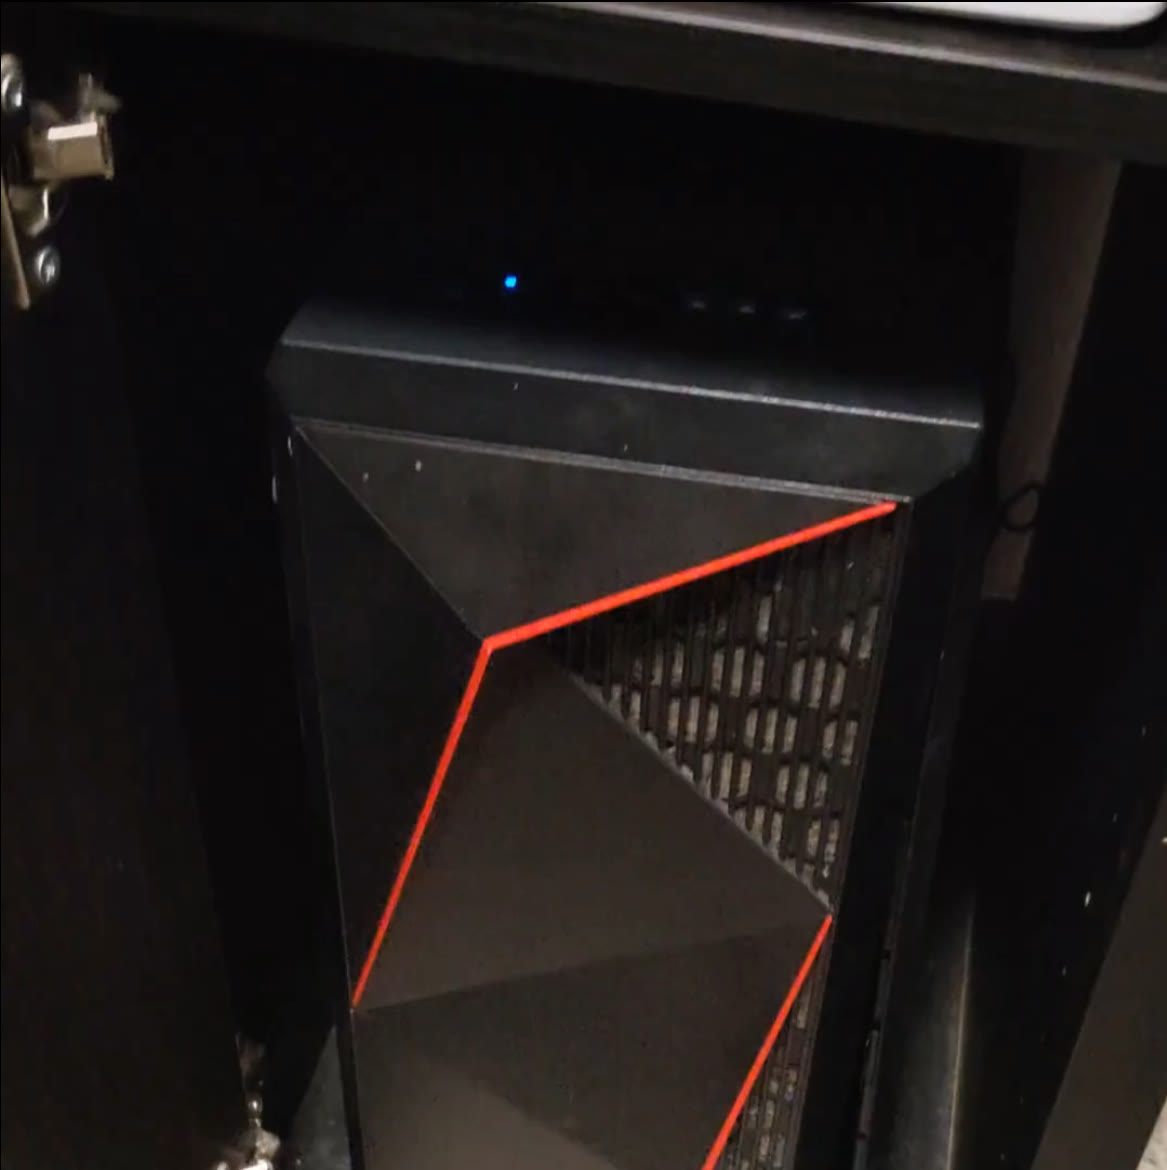
\includegraphics[width=0.95\textwidth, height=6.4cm,
              keepaspectratio]{captura_demo.png}};
            \fill[primary, opacity=0.7] (img.center) circle (0.7cm);
            \node[white, font=\Huge\bfseries] at (img.center) {$\blacktriangleright$};
          \end{tikzpicture}%
        }{video_demo.mp4}
      }{%
        \fbox{\parbox{0.85\textwidth}{\centering
          \vspace{2cm}
          \textcolor{primary}{\Huge $\blacktriangleright$}\\[0.2cm]
          {\large\bfseries\color{primary}VÍDEO DE DEMOSTRACIÓN}\\[0.1cm]
          {\footnotesize\color{darkgray}\texttt{captura\_demo.png} + \texttt{video\_demo.mp4}}
          \vspace{2cm}
        }}
      }
    \end{exampleblock}

    \column{0.45\textwidth}
    \begin{alertblock}{Protocolo de Contingencia}
      \scriptsize
      \textbf{Respaldo 1 — Local}\\[0.1cm]
      \centering
      \href{run:video_demo.mp4}{\beamergotobutton{Abrir archivo local}}\\[0.15cm]
      {\scriptsize\texttt{video\_demo.mp4}}

      \vspace{0.3cm}
      \textbf{Respaldo 2 — YouTube}\\[0.1cm]
      \centering
      \href{https://youtu.be/\_\_rJUlpLXP4}{\beamergotobutton{Ver en YouTube}}\\[0.15cm]
      {\scriptsize\texttt{youtu.be/\_\_rJUlpLXP4}}\\[0.2cm]
      \qrcode[height=0.8cm]{https://youtu.be/\_\_rJUlpLXP4}
    \end{alertblock}
  \end{columns}
\end{frame}

% ----------------------------------------------------------------------------
%  DIAPOSITIVA 26 — TELEGRAM + DASHBOARD
% ----------------------------------------------------------------------------
\begin{frame}{Demostración Práctica: Telegram + Dashboard}
  \sloppy
  \begin{columns}[T]
    \column{0.42\textwidth}
    \IfFileExists{\memoriaimg/hw_telegram_chat.jpg}{%
      
\includegraphics[height=4.3cm, keepaspectratio]{\memoriaimg/hw_telegram_chat.jpg}%
    }{%
      \fbox{\parbox{0.9\textwidth}{\centering\footnotesize [Chat Telegram]}}%
    }\\[0.1cm]
    {\footnotesize Conversación real con Luxe Core AI vía Telegram}

    \column{0.58\textwidth}
    \IfFileExists{\memoriaimg/hw_dashboard.png}{%
      
\includegraphics[height=4.3cm, keepaspectratio]{\memoriaimg/hw_dashboard.png}%
    }{%
      \fbox{\parbox{0.9\textwidth}{\centering\footnotesize [Dashboard OpenClaw]}}%
    }\\[0.1cm]
    {\footnotesize Dashboard web de OpenClaw (\texttt{http://192.168.1.50:18789})}
  \end{columns}

  \centering
  \footnotesize
  \textbf{Comandos en lenguaje natural}\\
  $\rightarrow$ interpretados en local\\
  $\rightarrow$ ejecución en hardware real.\\
  Ningún mensaje abandona la subred.
\end{frame}


% ============================================
%  BLOQUE VIII — CONCLUSIONES  (25–29)
% ============================================
% ============================================================================
%  BLOQUE VIII — DIAPOSITIVAS 27–31: CONCLUSIONES
% ============================================================================
\section{Conclusiones}

% ----------------------------------------------------------------------------
%  DIAPOSITIVA 27 — LOGROS VS RÚBRICA
% ----------------------------------------------------------------------------
\begin{frame}{Logros Alcanzados vs Rúbrica}
  \sloppy
  \footnotesize
  \begin{columns}[T]
    \column{0.52\textwidth}
    \begin{exampleblock}{Verificados sobre hardware real}
      \begin{itemize}
        \item \textbf{Arquitectura 3 capas escalable}
    \vspace{0.15cm}
        \item \textbf{Control local Tuya} (RF-03) — ON/OFF $<$2 s
        \item \textbf{Lectura BLE Xiaomi} (RF-02) — GATT sin nube
        \item \textbf{FanLamp F8808} (RF-04) — 11 comandos
        \item \textbf{Model Router v2} — 462 patrones, 92\% cobertura
        \item \textbf{SelfHealManager} — 24 h sin caídas
        \item \textbf{Canales Telegram + Dashboard} operativos
      \end{itemize}
    \end{exampleblock}

    \column{0.48\textwidth}
    \begin{block}{Estado de los módulos}
      \resizebox{\columnwidth}{!}{%
      \begin{tabular}{lcc}
        \toprule
        \textbf{Módulo} & \textbf{Estado} & \textbf{Obs.} \\
        \midrule
        Tuya Plug & \checkmark & Air-gapped \\
        BLE Xiaomi & \checkmark & GATT directo \\
        FanLamp & \checkmark & 11 comandos \\
        OpenClaw & \checkmark & Puerto 18789 \\
        Model Router & \checkmark & 3 niveles \\
        ESP32 HVAC & Pendiente & Firmware C++20 \\
        \bottomrule
      \end{tabular}}%

      \vspace{0.15cm}
      \centering
      \textbf{5/6 módulos. 0 € en licencias.}
    \vspace{0.15cm}
    \end{block}
  \end{columns}
\end{frame}

% ----------------------------------------------------------------------------
%  DIAPOSITIVA 28 — TRABAJO FUTURO CORTO PLAZO
% ----------------------------------------------------------------------------
\begin{frame}{Trabajo Futuro: Corto Plazo}
  \sloppy
  \begin{columns}[T]
    \column{0.5\textwidth}
    \begin{alertblock}{Firmware HVAC (ESP32 + LIN)}
      \footnotesize
      \textbf{Prioridad inmediata} — Hardware adquirido.\\
      \texttt{esphome-fujitsu-halcyon} como base. \textbf{2--3 semanas}
    \end{alertblock}

    \begin{alertblock}{Eliminar puente ESP32}
      \footnotesize
      Control BLE directo con \texttt{bleak}.
      Elimina punto único de fallo. \textbf{1--2 semanas}
    \end{alertblock}

    \begin{exampleblock}{\textit{Streaming} SSE Tier~2}
      \footnotesize
      Mostrar palabras conforme se generan. \textbf{1--2 semanas}
    \end{exampleblock}

    \column{0.5\textwidth}
    \begin{exampleblock}{Bucle de control con OpenClaw}
      \footnotesize
      Conectar sensores BLE, Tuya y FanLamp al orquestador.
      \textbf{1--2 semanas}
    \end{exampleblock}

    \begin{exampleblock}{Containerización Docker}
      \footnotesize
      \texttt{docker-compose} para replicabilidad total.
      \textbf{1--2 semanas}
    \end{exampleblock}

    \begin{block}{Total corto plazo}
      \footnotesize
      5 líneas. Estimación: \textbf{5--10 semanas}.
    \end{block}
  \end{columns}
\end{frame}

% ----------------------------------------------------------------------------
%  DIAPOSITIVA 29 — TRABAJO FUTURO LARGO PLAZO
% ----------------------------------------------------------------------------
\begin{frame}{Trabajo Futuro: Medio y Largo Plazo}
  \begin{columns}[T]
    \column{0.5\textwidth}
    \footnotesize
    \textbf{Medio plazo (meses)}
    \vspace{0.15cm}
    \begin{itemize}
      \item \textbf{Expansión \textit{dashboard}:}\\
      {\scriptsize Analíticas energéticas, histórico ASHRAE 55 — 1--2 meses}
      \item \textbf{Expansión sensorial:}\\
      {\scriptsize Sensor presencia LD2410, micrófono/altavoz — 1--2 meses}
      \item \textbf{Base de datos vectorial:}\\
      {\scriptsize Qdrant o ChromaDB para recuperación semántica — 2--3 meses}
      \item \textbf{Memoria conversacional:}\\
      {\scriptsize \textit{Embeddings} con \texttt{bge-m3}, referencias implícitas — 2--3 meses}
    \end{itemize}

    \column{0.5\textwidth}
    \footnotesize
    \textbf{Largo plazo (investigación)}
    \vspace{0.15cm}
    \begin{itemize}
      \item \textbf{Aprendizaje adaptativo:}\\
      {\scriptsize \textit{Reinforcement learning} para hábitos del usuario — varios meses}
      \item \textbf{Nuevos protocolos:}\\
      {\scriptsize Zigbee, Z-Wave $\rightarrow$ más dispositivos — varios meses}
      \item \textbf{Re-evaluación de modelos:}\\
      {\scriptsize Qwen3.5 (sin \textit{thinking}), Llama 4, DeepSeek — continuo}
      \item \textbf{\textit{Fine-tuning} clasificador:}\\
      {\scriptsize Ajuste con datos reales de uso doméstico — varios meses}
    \end{itemize}
  \end{columns}
\end{frame}

% ----------------------------------------------------------------------------
%  DIAPOSITIVA 30 — REFLEXIÓN PRIVACIDAD
% ----------------------------------------------------------------------------
\begin{frame}{Privacidad por Diseño: Reflexión}
  \footnotesize
  \begin{columns}[T]
    \column{0.55\textwidth}
    \begin{block}{El principio fundamental}
      \centering
      \normalsize\textbf{La tecnología del hogar no debería\\[0.05cm]
      exigir ceder la privacidad a cambio de comodidad.}
    \end{block}

    \textbf{Lo que hemos comprobado:}
    \vspace{0.15cm}
    \begin{itemize}
      \item Es posible tener \textbf{ambas cosas} con hardware de consumo
      \item La arquitectura \textit{air-gapped} es viable y verificable
      \item Los modelos pequeños en local \textbf{funcionan}
    \vspace{0.15cm}
      \item La interoperabilidad no depende de la nube: depende del software
    \end{itemize}

    \column{0.45\textwidth}
    \begin{exampleblock}{Más allá de lo técnico}
      La decisión de mantener todo en local fue una cuestión de principios.
    \end{exampleblock}

    \begin{alertblock}{Y en pocos años...}
      Modelos ligeros con capacidad cercana a los grandes cloud:\\
      \centering
      \textit{«¿se puede en local?»} $\rightarrow$
      \textbf{«¿por qué en la nube?»}
    \vspace{0.15cm}
    \end{alertblock}
  \end{columns}
\end{frame}

% ----------------------------------------------------------------------------
%  DIAPOSITIVA 31 — CIERRE FORMAL
% ----------------------------------------------------------------------------
{
\setbeamertemplate{footline}{}
\setbeamertemplate{frametitle}{}

\begin{frame}[plain]

  \begin{tikzpicture}[remember picture, overlay]

    % --- Esquina superior derecha (decoración institucional) ---
    \node[anchor=north east, inner sep=0pt] at (current page.north east) {%
      \IfFileExists{\memoriaimg/topRightCorner.pdf}{%
        
\includegraphics[width=2.5cm]{\memoriaimg/topRightCorner.pdf}%
      }{}%
    };

    % --- Esquina inferior izquierda (decoración institucional) ---
    \node[anchor=south west, inner sep=0pt] at (current page.south west) {%
      \IfFileExists{\memoriaimg/bottomLeftCorner.pdf}{%
        
\includegraphics[width=2.5cm]{\memoriaimg/bottomLeftCorner.pdf}%
      }{}%
    };

    % --- Escudo Informática + Logo UCO ---
    \node[anchor=south east, xshift=-0.8cm, yshift=0.8cm] at (current page.south east) {%
      \IfFileExists{\memoriaimg/escudo_informatica.jpg}{%
        
\includegraphics[height=1.0cm]{\memoriaimg/escudo_informatica.jpg}%
      }{}%
      \hspace{0.2cm}%
      \IfFileExists{\memoriaimg/logoUCO.pdf}{%
        
\includegraphics[height=1.0cm]{\memoriaimg/logoUCO.pdf}%
      }{}%
    };

    % --- Línea accent superior ---
    \draw[accent, line width=3pt]
      (current page.north west) -- (current page.north east);

  \end{tikzpicture}

  \vspace*{2.5cm}

  {\parskip=0pt
  \begin{center}
    {\Large\bfseries\color{primary}Luxe Core AI}

    \vspace{1.0cm}

    {\Huge\bfseries\color{primary}Muchas gracias por su atención.}

    \vspace{0.6cm}

    {\normalsize\color{darkgray}
     Quedo a disposición del ilustre tribunal\\
     para resolver las cuestiones que consideren oportunas.}

    \vfill

    \makebox[4cm]{\hrulefill}

    \vspace{0.2cm}
    {\normalsize\color{darkgray}Jesús Fernández López}\\[0.08cm]
    {\normalsize\color{darkgray}Grado en Ing. Informática — UCO}\\[0.06cm]
    {\normalsize\color{darkgray}Junio 2026}
  \end{center}}

\end{frame}
}


\end{document}
